% !TeX program = pdfLaTeX
\documentclass[12pt]{article}
\usepackage{amsmath}
\usepackage{graphicx,psfrag,epsf}
\usepackage{enumerate}
\usepackage{natbib}
\usepackage{textcomp}
\usepackage[hyphens]{url} % not crucial - just used below for the URL
\usepackage{hyperref}

%\pdfminorversion=4
% NOTE: To produce blinded version, replace "0" with "1" below.
\newcommand{\blind}{0}

% DON'T change margins - should be 1 inch all around.
\addtolength{\oddsidemargin}{-.5in}%
\addtolength{\evensidemargin}{-.5in}%
\addtolength{\textwidth}{1in}%
\addtolength{\textheight}{1.3in}%
\addtolength{\topmargin}{-.8in}%

%% load any required packages here



% tightlist command for lists without linebreak
\providecommand{\tightlist}{%
  \setlength{\itemsep}{0pt}\setlength{\parskip}{0pt}}



\usepackage{booktabs}
\usepackage{longtable}
\usepackage{array}
\usepackage{multirow}
\usepackage{wrapfig}
\usepackage{float}
\usepackage{colortbl}
\usepackage{pdflscape}
\usepackage{tabu}
\usepackage{threeparttable}
\usepackage{threeparttablex}
\usepackage[normalem]{ulem}
\usepackage{makecell}
\usepackage{xcolor}

\begin{document}


\def\spacingset#1{\renewcommand{\baselinestretch}%
{#1}\small\normalsize} \spacingset{1}


%%%%%%%%%%%%%%%%%%%%%%%%%%%%%%%%%%%%%%%%%%%%%%%%%%%%%%%%%%%%%%%%%%%%%%%%%%%%%%

\if0\blind
{
  \title{\bf Climate Change and Aging: A systematic Review}

  \author{
        Mathew E. Hauer \thanks{The authors gratefully acknowledge
\ldots{}} \\
    Department of Sociology, Florida State University\\
     and \\     Kyle Rose \\
    Department of Sociology, Florida State UniversityW\\
      }
  \maketitle
} \fi

\if1\blind
{
  \bigskip
  \bigskip
  \bigskip
  \begin{center}
    {\LARGE\bf Climate Change and Aging: A systematic Review}
  \end{center}
  \medskip
} \fi

\bigskip
\begin{abstract}
In this systematic review, we analyze the literature through Web of
Science's SCI-Expanded containing the words ``aging'' or ``aged'' and
``climate change'' and receiving at least four citations per year since
publication (n = 607 articles). After discarding irrelevant articles
(ie, ``aging infrastructure''), the 177 remaining articles
overwhelmingly (60\%) fall into two categories: temperature/mortality
(n= 85; 48\%) and temperature/morbidity (n = 22; 12\%). However, many
other important climate topics related to aging remain underdeveloped.
Notably, adaptation (n = 8; 6\%), vulnerability (n = 5; 4\%),
emissions/mitigation (n = 4; 3\%), drought and mortality (n = 1; 0.7\%),
food security (n = 1; 0.7\%), and climate perceptions (n = 0) remain
understudied. Furthermore, more than half of the studies were conducted
in the United States (n = 31; 18\%), China (n = 35; 20\%), Globally (n =
21; 12\%), and Australia (n = 12; 7\%), suggesting a paucity of
information in the Global South (n = 11) where climate impacts will be
greatest. There were more studies specifically on Spain (n = 5) than
specifically on the entire African continent (n = 4). Finally, 18
articles (13\%) offered projections in some form, most to the middle of
the century. Gerontologists and aging scientists should look beyond the
relationship between heat and mortality to offer a more holistic view of
aging and climate change. {[}Sentence about Geography{]}. Prospective
analyses, as opposed to retrospective, could shed additional light on
the link between aging and climate change.
\end{abstract}

\noindent%
{\it Keywords:} 3 to 6 keywords, that do not appear in the title
\vfill

\newpage
\spacingset{1.45} % DON'T change the spacing!

\hypertarget{introduction}{%
\section{Introduction}\label{introduction}}

Two seemingly immutable trends will crash head-on during this century:
the global populace will continue to age and global climate change
impacts will worsen as the century progresses. By the end of the
century, when climate change impacts will be considerably more intense
than today, the Global populace exposed to these impacts will be
decidedly older, amplifying climate change impacts. Many of the
anticipated impacts from climate change disproportionately impact the
elderly versus younger, more vigorous age groups making these two trends
particularly potent when taken together.

Consider this: the Global populace will age universally. The global
population aged 75+ is expected to grow from 271M people today to nearly
1.4B people by 2100 \citep{division_wpp2017}. Today, only Japan, Italy,
and Germany have median ages in excess of 50. But by 2100, 54\% of
countries will be as old as or older than these countries are today.
These demographic trends are well known
\citep{lutz2008coming, beard2016world}.

While the global, dramatic aging shift occurs, the world will continue
to warm. Climate projections suggest global temperatures are likely
increase more than 3 degrees Celsius by 2100 compared to the
pre-industrial period \citep{arias2021climate}. These temperature
increases will likely usher in increasingly frequent and destructive
extreme weather events, more frequent droughts and wildfire risks,
extreme heat, and substantially increase the burden on health services
\citep{portner2022climate}. Low-lying coastal areas will experience
increased coastal flooding and the submergence of many coastal cities
appears likely \citep{kulp2019new}. Climate change will make the world
of 2100 considerably more precarious compared to today, a precarity
amplified by a globally aging populace.

Nearly every climate impact is heightened by age due to the older
people's social vulnerability and physiological susceptibility. Older
adults have increased social vulnerability to psychological stresses due
to environmental change, reduced ability to adapt, limited
transportation, reduced mobility, smaller social networks, lower
incomes, chronic health problems, social isolation, cognitive decline,
and general fragility \citep{kovats2008heat}. This elevated social
vulnerability combines with older adult's increased physiological
vulnerability to extreme heat and cold, extreme weather events, and
infectious diseases to create a biophysical cocktail of potential
catastrophe.

Additionally, climate change and aging intersect in multiple ways,
beyond just climate impacts. Older adults play important roles in the
mitigation or reduction of carbon emissions
\citep{oneill_global_2010, buchs_who_2013}. Adaptation to climate
impacts greatly vary among older populations
\citep{huang_is_2011, guo_high_2012} and perceptions of climate risks
can serve as barriers to effective adaptation
\citep{hansen_perceptions_2011, abrahamson_perceptions_2008}. Yet, as we
show in this article, most research concerning aging and climate change
tends to focus on the impact of extreme temperatures on older
populations. A more holistic view of the aging and climate change
literature could shed light on the varied relationships between older
adults and global environmental change.

In this article, we conduct a systematic review of the literature
surrounding climate change and aging.

\hypertarget{methods-and-materials}{%
\section{Methods and Materials}\label{methods-and-materials}}

We use a systematic literature review to assess the literature on
climate change and aging.

\hypertarget{document-selection}{%
\subsection{Document selection}\label{document-selection}}

We used a keyword search on Clarviate's Web of Science-expanded search
engine using the Boolean operator ``TS=(aging OR aged OR elderly) AND
TS=(``climate change'').'' We selected Web of Science due to its
comprehensive scientific coverage of peer-reviewed literature. We
conducted the search on September 7, 2022. This search retrieved an
initial universe of 16,828 articles. We filtered these results to
include articles of relatively high impact, defined subjectively as
those articles with at least four citations per year (n = 3,852). To
further isolate those articles pertaining to aging and climate change,
we further restricted our search to those articles containing the words
(aging or aged or elderly) in the abstract (n = 607).

We then reviewed these articles for relevance, discarding articles
concerning ``aging infrastructure'' or ``aging forests'' to isolate
articles on human aging and climate change. This yielded a total of 177
articles included in this systematic review
(\textbf{\autoref{fig-diagram}}).

\begin{figure}
\centering
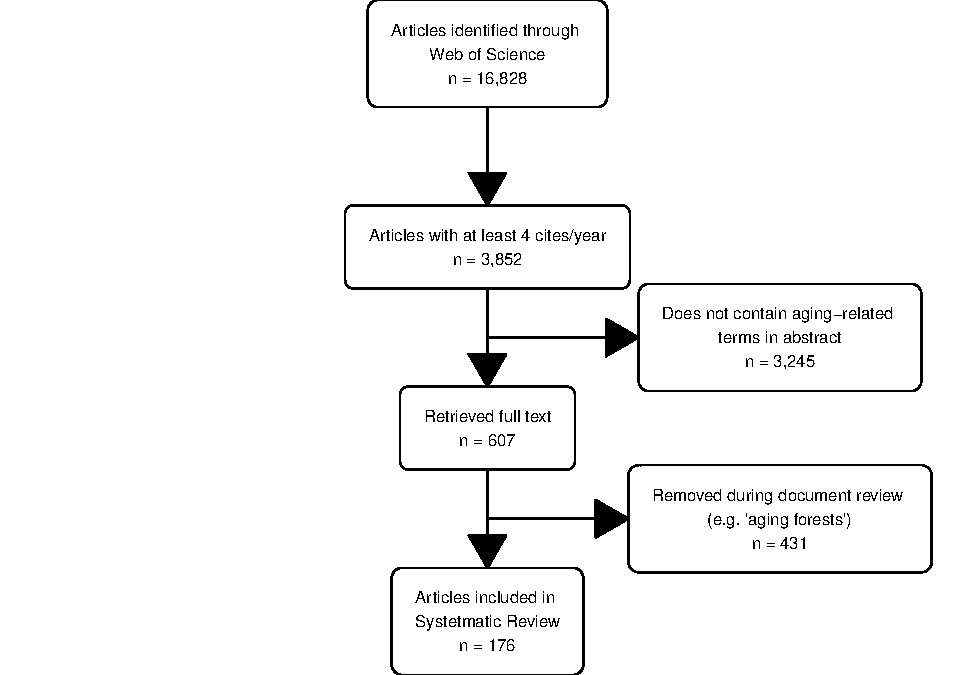
\includegraphics{MainDocument_files/figure-latex/figureflowdiagram-1.pdf}
\caption{PRISMA Flow Diagram. \label{fig-diagram}}
\end{figure}

\hypertarget{document-review}{%
\subsection{Document review}\label{document-review}}

Following our document selection and screening, 607 articles were
retained for full review. We developed a questionnaire to survey these
articles to document and characterize the primary topics of climate
change. We developed this questionnaire to standardize the analysis,
produce descriptive statistics, and examine trends. We coded all papers
based on (1) the primary and (2) secondary climate effect studied, (3)
the climate impact type (sensitivity, vulnerability, or exposure), (4)
the climate impact studied (morbidity, mortality, etc.), if the article
concerned (5) mitigation, (6) adaptation, (7) or perceptions, if the
article included a projection (8), the historic time period (9), and the
general area the study was conducted (10). Additionally, we gathered
general information on authorship, publication year, and citation
counts. We conducted an extensive full-text review of all (n = 607)
articles using this questionnaire. We assessed the primary finding in
articles where multiple climate impact types or climate impacts were
studied.

\hypertarget{analysis}{%
\subsection{Analysis}\label{analysis}}

All (n = 16,828) articles were retained for validation. All data were
entered into an Excel spreadsheet. We used R to analyze the data and to
produce descriptive statistics and visualizations.

\hypertarget{data-availability}{%
\section{Data Availability}\label{data-availability}}

The underlying computer code and data that support the findings of this
study are available in the Supplementary Material and have been
deposited in Zenodo (DOI).

\bibliographystyle{agsm}
\bibliography{bibliography.bib}


\end{document}
